\documentclass[a4paper,10pt]{article}

\usepackage[english]{babel}
\usepackage{graphicx}
\usepackage[colorlinks, allcolors=black]{hyperref}
\usepackage{geometry}
\geometry{tmargin=3cm, bmargin=2.2cm, lmargin=2.2cm, rmargin=2cm}
\usepackage{todonotes} %Used for the figure placeholders

% Your name and student number must be filled in on the title page found in
% titlepage.tex.

\begin{document}
\begin{titlepage}
    \newpage
    \thispagestyle{empty}
    \frenchspacing
    \hspace{-0.2cm}
    
\includegraphics[height=3.4cm]{sedes}
    \hspace{0.2cm}
    \rule{0.5pt}{3.4cm}
    \hspace{0.2cm}
    \begin{minipage}[b]{8cm}
        \Large{Katholieke\newline Universiteit\newline Leuven}\smallskip\newline
        \large{}\smallskip\newline
        \textbf{Department of\newline Computer Science}\smallskip
    \end{minipage}
    \hspace{\stretch{1}}
    \vspace*{3.2cm}\vfill
    \begin{center}
        \begin{minipage}[t]{\textwidth}
            \begin{center}
                \LARGE{\rm{\textbf{\uppercase{Document Processing}}\\ADD
                application}}\\
                \Large{\rm{Software Architecture (H09B5a and H07Z9a) -- 
                Part 2a}}
            \end{center}
        \end{minipage}
    \end{center}
    \vfill
    \hfill\makebox[8.5cm][l]{%
        \vbox to 7cm{\vfill\noindent
            {\rm \textbf{Student A (r123456)}}\\
            {\rm \textbf{Student B (r987654)}}\\[2mm]
            {\rm Academic year 2014--2015}
        }
    }
\end{titlepage}


\tableofcontents
\newpage

\section{Introduction}\label{sec:introduction}
The goal of this project was to develop  an architecture for a system for document processing. This part of the project consisted of 
\section{Overview}\label{sec:overview}
\subsection{Architectural decisions}
Briefly discuss your architectural decisions for each non-functional
requirement.
Pay attention to the solutions that you employed (in your own terms or using
tactics and/or patterns).

\paragraph{ReqX\@: requirement name} Provide a brief discussion of the
decisions related to \emph{ReqX}.\\
\emph{Employed tactics and patterns: List all patterns and tactics used to
    achieve ReqX, if any.}

\subsection{Discussion}
Use this section to discuss your architecture in retrospect.
For example, what are the strong points of your architecture?
What are the weak points? Is there anything you would have done otherwise with
your current experience?
Are there any remarks about the architecture that you would give to your
customers?
Etc.

\section{Attribute-driven design documentation}\label{sec:add}
\subsection{Decomposition 1: eDocs (X1, Y3, UCa, UCb, UCc)}
\subsubsection{Module to decompose}
In the first run, the eDocs System is decomposed as a whole\subsubsection{Selected architectural drivers}
The non-functional drivers for this decomposition are:

\begin{itemize}
    \item \emph{X1}: name
    \item \emph{Y3}: name
\end{itemize}

The related functional drivers are:

\begin{itemize}
    \item \emph{UCa}: name
    \item \emph{UCb}: name
    \item \emph{UCc}: name
\end{itemize}

\paragraph{Rationale}
A short discussion of why these drivers were selected for this decomposition.

\subsubsection{Architectural design}
\paragraph{Topic}
Discussion of the solution selected for (a part of) one of the architectural
drivers.

\subsubsection*{Alternatives considered}
\paragraph{Alternatives for solution}
A discussion of the alternative solutions and why that were not selected.

\subsubsection{Instantiation and allocation of functionality}
\paragraph{Decomposition}
Main aspects of the resulting decomposition.

\subparagraph{ModuleB}
Per introduced component a paragraph describing its responsibilities.

\subparagraph{ModuleC}
Per introduced component a paragraph describing its responsibilities.

\begin{figure}[!htp]
    \centering
    %\includegraphics[width=0.8\textwidth]{}
    \missingfigure[figwidth=0.8\textwidth]{Component-and-connector diagram}
    \caption{Component-and-connector diagram of this decomposition.
        }\label{fig:it1-cc_main}
\end{figure}

\paragraph{Behaviour}
If needed and explanation of the behaviour of certain aspects of the design so
far.

\begin{figure}[!htp]
    \centering
    %\includegraphics[width=0.8\textwidth]{}
    \missingfigure[figwidth=0.8\textwidth]{Sequence diagram}
    \caption{Sequence diagram illustrating a key behavioural aspect.
        }\label{fig:it1-seq_aspect1}
\end{figure}

\paragraph{Deployment}
Rationale of the allocation of components to physical nodes.

\begin{figure}[!htp]
    \centering
    %\includegraphics[width=0.8\textwidth]{}
    \missingfigure[figwidth=0.8\textwidth]{Deployment diagram}
    \caption{Deployment diagram of this decomposition.
        }\label{fig:it1-depl_main}
\end{figure}

\subsubsection{Interfaces for child modules}
\subsubsection*{PDSDB}
\begin{itemize}
    \item DocumentMgmt
    \begin{itemize}
        \item \texttt{void storeDocument(DocumentId id, Document doc, MetaData md)}
        \begin{itemize}
            \item Effect: The \texttt{PDSDB} will store the given document\texttt{doc} together with the provided metadata \texttt{md}.
            \item Exceptions:  None 
        \end{itemize}

        \item \texttt{Tuple<Document, MetaData> getDocument(DocumentId id)}
        \begin{itemize}
            \item Effect: Describe the effect of calling this operation.
            \item Exceptions: None
         \end{itemize}
         
         \item \texttt{void markReceived(DocumentId id)}
        \begin{itemize}
            \item Effect: Describe the effect of calling this operation.
            \item Exceptions: None
         \end{itemize}
    \end{itemize}
\end{itemize}

\subsubsection{Data type definitions}
Describe per complex data type used in the interfaces what it represents.

\paragraph{returnType} This data element represents X.

\paragraph{ParamType} This data element represents Y.

\subsubsection{Verify and refine}
This section describes per component which (parts of) the remaining
requirements it is responsible for.

\paragraph{ModuleB}
\begin{itemize}
    \item \emph{Z1}: name
    \item \emph{UCd}: name
\end{itemize}

\paragraph{ModuleC}
\begin{itemize}
    \item \emph{UCba}: name\\Description which part of the original use case is
        the responsibility of this component.
\end{itemize}


\
\subsection{Decomposition 2: OtherFunctionality(P2, Av2b, UC12, UC13, UC14, UC15)}
\subsubsection{Module to decompose}
In this run we decompose \texttt{Otherfunctionality}.

\subsubsection{Selected architectural drivers}
The non-functional driver for this decomposition is:

\begin{itemize}
    \item \emph{P2}: Document lookups
    \item \emph{Av2b}: Temporary storage for PDSDB
\end{itemize}

The related functional drivers are:

\begin{itemize}
    \item \emph{UC12}: Consult personal document store
    \item \emph{UC13}: Search documents in personal document store
    \item \emph{UC14}: Consult document in personal document store
    \item \emph{UC15}: Download document via unique link
\end{itemize}

\paragraph{Rationale}
P2 and Av2b were chosen because their priorities are amongst the highest ones of all remaining non-functional drivers and the domains on which their focus lies complement the previous decomposition perfectly.

\subsubsection{Architectural design}

\paragraph{Link mapping}
In order to support document lookups via links, which are either unique (unregistered recipient) or part of a notification e-mail (registered recipient), the \texttt{UserFacade} is concerned with the mapping of each incoming link request to the appropriate document, which is either located in the \texttt{PDSDB} (for registered recipients) or in the \texttt{DocumentDB} (for unregistered recipients). The mappings themselves are stored in the \texttt{MappingDB} component and are fetched by the \texttt{UserFacade} when needed.

\paragraph{Dedicated DocumentDB and LinkMappingDB for P2}
Since a large number of document lookups and downloads should not affect the performance of other functionality of the system, both link mappings and documents are stored in dedicated databases, each deployed on a different node. This decision ensures that documents can be looked up via the personal document store or a notification in a timely fashion, because it prohibits either of those two components to be a bottleneck in the document lookup process. Since, according to the previous decomposition, the \texttt{PDSDB} is deployed on a separate node too, this component's performance is already satisfactory and no changes need to be made to improve it.

\paragraph{Sharding for DocumentDB for P2}
In order to improve performance of the \texttt{DocumentDB}, we chose to partition this database into multiple shards. This approach was driven by the need for fast response time while keeping in mind the high storage cost for documents. More precisely, a \texttt{ShardingManager} is responsible for reading and writing all documents in one of the \texttt{DocumentDBShards}, making sure that every document is stored only once. This sharding technique provides roughly the same advantages in response time as active replication, but is significantly less costly when it comes to storage capacity.
Note that there must also be a (sub)component monitoring all requests to the shards, in order to throttle excessive requests when necessary. Since this is a rather simple task and the (sub)component must be aware of the details concerning the sharding architecture to efficiently fulfil its purpose, this functionality is delegated to the \texttt{ShardingManager} itself. Finally, this \texttt{ShardingManager} is also responsible for implicitly pinging all \texttt{DocumentDBShards} upon reading and writing in them.

\paragraph{DocumentStorageCache for Av2b}
This component temporarily stores the IDs of all generated documents that are to be delivered through the personal document store during downtime of the \texttt{PDSDB} component up to a maximum of 3 hours. When the latter component turns operational again, the \texttt{DocumentStorageManager} retrieves all documents and their corresponding meta data from the \texttt{DocumentDB} using the previously mentioned IDs and subsequently stores them in the \texttt{PDSDB}. Note that the recipient therefore perceives a maximum total downtime of 3 hours plus the time needed for the \texttt{DocumentStorageManager} to transfer all documents and meta data that the cached IDs refer to. \\
Note that the \texttt{DocumentDB} and the \texttt{PDSDB} store documents in exactly the same way, both including the document itself, its meta data and its ID, although there is no need for the meta data in the former database. This storage tactic ensures that the \texttt{DocumentStorageManager} does not have to fetch or convert any information when transferring documents between both databases, making the transfer as efficient as possible. This does not introduce any overhead to the storage system, since the meta data is but a fraction of the document data. \\
Finally, we would like to stress that the \texttt{DocumentStorageManager} implicitly pings the \texttt{PDSDB} when storing document data in it. The echo message then, in turn, consists of the write confirmation that is subsequently received. If one of those writes should fail, all subsequent writes are converted into document ID writes to the aforementioned cache. Upon revival of the \texttt{PDSDB}, this database will send a single heartbeat to the \texttt{DocumentStorageManager}, causing this component to begin transferring the missing document data. Once all cached document IDs are processed, subsequent writes to the \texttt{PDSDB} will no longer be redirected through the \texttt{DocumentStorageCache}.

\subparagraph{UserFacade}
We introduce this component to be able to distinguish between registered recipients and unregistered recipients in the first steps of the document lookup process. The \texttt{UserFacade} also maps incoming links to documents that are located either in the \texttt{PDSDB} or in the \texttt{DocumentDB} by first fetching the correct mapping from the \texttt{LinkMappingDB} mentioned above. Another responsibility of the \texttt{UserFacade} is marking documents as received, since this is the last internal component through which the document is passed before the requesting recipient actually receives it and failure of another component in the document lookup pipeline can no longer prevent this from happening.

\subparagraph{PDSFacade}
This component handles all read requests that are intended for the personal document store. This extra level of indirection calculates and aggregates all intermediate query results as to relieve the \texttt{PDSDB} of this burden, which is also the reason why both components are best deployed on different nodes. Upon querying the personal document store, this component first collects the recipient's documents' meta data and subsequently performs queries on this collection. This approach introduces no significant overhead, because only those documents that are needed, will be fetched in their entirety. It is also the responsibility of the \texttt{PDSFacade} to check the recipient's ID against the recipient ID that can be retrieved from the document meta data and to only pass on those documents for which they are a match.

\subparagraph{DocumentStorageManager}
The storage of documents is handled by the \texttt{DocumentStorageManager}, which receives generated documents from the intermediary \texttt{OtherFunctionality2} component and stores them in either the \texttt{DocumentDB} (for unregistered recipients) or in both the \texttt{DocumentDB} and the \texttt{PDSDB} (for registered recipients) according to the method that is invoked on it. The necessity for this component follows from the fact that synchronisation is needed between the two storage components mentioned above. Note that the PDSDocMgmt interface in the \texttt{PDSDB} component now requires an extra method to save documents.

\subsubsection*{Alternatives considered}

\paragraph{Alternative for DocumentStorageCache}
We could just as well do without the previously introduced \texttt{DocumentStorageCache} by letting the \texttt{DocumentStorageManager} actively look for documents in the \texttt{DocumentDB} that are not yet, but should be, present in the \texttt{PDSDB} upon revival of the \texttt{PDSDB}. A clear advantage of this approach is that the downtime of the \texttt{PDSDB} component is no longer restricted by the aforementioned 3-hour cache. An important disadvantage, however, lies in the fact that the \texttt{DocumentStorageManager} is burdened with a significant amount of extra work and will require more expensive hardware to cope with this. Since the support for a longer downtime of the \texttt{PDSDB} is out of scope, this approach was not chosen.

%Merk op: als alternatief hadden we gedacht aan GEEN actieve heartbeat vanuit de PDSDB bij het online komen, maar bij een schrijfpoging naar de PDSDB als impliciete ping wanneer er een document opgeslagen wordt. Het probleem hierbij is dat wanneer er al even geen documenten genereerd zijn maar er toch noch documentreferenties in de cache zitten en op dat moment de PDSDB online komt, een registered recipient die documenten niet kan opvragen.

\subsubsection{Instantiation and allocation of functionality}
\paragraph{Decomposition}
Figure \ref{fig:decomp2} shows the components resulting from the decomposition in this run. Extra attention is required concerning the \texttt{DocumentDBShard}. This component actually represents multiple instances, each containing a different partition of the document data to accommodate for parallel lookups in different partitions while minimizing storage costs.
The responsibilities of the resulting components are as follows:

\subparagraph{DocumentDB}
Responsible for storing all generated documents.

\subparagraph{ShardingManager}
Responsible for managing all reads and writes to the \texttt{DocumentDBShards}.

\subparagraph{DocumentDBShard}
Responsible for storing a partition of the documents in the \texttt{DocumentDB}

\subparagraph{LinkMappingDB}
Responsible for storing the mappings between links and document locations.

\subparagraph{UserFacade}
We introduce this component to be able to distinguish between registered recipients and unregistered recipients in the first steps of the document lookup process. The \texttt{UserFacade} also maps incoming links to documents that are located either in the \texttt{PDSDB} or in the \texttt{DocumentDB} by first fetching the correct mapping from the \texttt{LinkMappingDB} mentioned above. Another responsibility of the \texttt{UserFacade} is marking documents as received, since this is the last internal component through which the document is passed before the requesting recipient actually receives it and failure of another component in the document lookup pipeline can no longer prevent this from happening.

\subparagraph{PDSFacade}
This component handles all read requests that are intended for the personal document store. This extra level of indirection calculates and aggregates all intermediate query results as to relieve the \texttt{PDSDB} of this burden, which is also the reason why both components are best deployed on different nodes. Upon querying the personal document store, this component first collects the recipient's documents' meta data and subsequently performs queries on this collection. This approach introduces no significant overhead, because only those documents that are needed, will be fetched in their entirety. It is also the responsibility of the \texttt{PDSFacade} to check the recipient's ID against the recipient ID that can be retrieved from the document meta data and to only pass on those documents for which they are a match.

\subparagraph{DocumentStorageManager}
The storage of documents is handled by the \texttt{DocumentStorageManager}, which receives generated documents from the intermediary \texttt{OtherFunctionality2} component and stores them in either the \texttt{DocumentDB} (for unregistered recipients) or in both the \texttt{DocumentDB} and the \texttt{PDSDB} (for registered recipients) according to the method that is invoked on it. The necessity for this component follows from the fact that synchronisation is needed between the two storage components mentioned above. Note that the PDSDocMgmt interface in the \texttt{PDSDB} component now requires an extra method to save documents.

\subparagraph{DocumentStorageCache}
Responsible for temporarily storing the IDs of all generated documents that are to be delivered through the personal document store during downtime of the \texttt{PDSDB} component.

\subparagraph{OtherFunctionality2}
Encapsulates requirements that are not tackled in this run and cannot be assigned to other introduced components.





\subsubsection*{UserFacade}
The \texttt{UserFacade} provides three interfaces to the recipient: \textit{AuthN} for authentication, \textit{UniqueLinkMgmt} for document lookups via unique links and \textit{PDSDBMgmt} for access to the personal document store. Links to documents in the PDSDB that are part of a notification e-mail are therefore handled by the latter, in which case the \texttt{UserFacade} also needs to perform a check to see if the requesting recipient is registered in the eDocs system.

\subsubsection{Verify and refine}
This section describes per component which (parts of) the remaining
requirements it is responsible for.

Residual Av2b2 : TIJDIGE notification AAN DE USER

USE CASE 12: residual drivers: het opslaan van de recipient id's in de pdsdb --> hoort bij deliveryfunctionality. --> voorlopig verondersteld dat recipientID in meta data zit die samen met doc opgeslagen wordt in zowel docDB als PDS
Ook het inloggen (authenticatie).
USE CASE 13:  residual drivers: we veronderstellen dat de DocumentStorageManager metadata bij elk document opslaat, like the name of the sender, the data range in which the document should be received and the document type --> hoort bij deliveryfunctionality.
The metadata is saved in both the pdsdb en database components, because when a user registers, this metadata has to be copied form the one to the other. Dit is om gemakkelijk de documenten in de pdsdb te kunnen zoeken.
USE CASE 14:  residual driver: mark as received, puntje 3. --> beter te doen bij de deliveryfunctionality
USE CASE 15:  residual driver: tracking.

\paragraph{LinkManager} VOORLOPIG NIET NODIG IN DEZE DECOMPOSITIE

Motivatie voor LinkManager: Checks expiration date ALS DAT NODIG IS--> reason: links naar de pdsdb vervallen niet (zolang de gebruik geregistreerd is)
LinkManager maps link to (document ID, place where the document is stored)-pairs --> REASON: the unique link has two possible sources: an e-mail to an unregistered recipient or an email to a registered recipient. For an unregistered recipient, the RecipientFacade must look with the documentid for the document in the documentDB. For a registered recipient, the RecipientFacade must look with the documentid for the document  in the PDSDB. (Mogelijk een boolean ofzo)

Does NOT do mapping removal after x years --> there has to be a notification when the link has expired

\section{Client-server view (UML Component diagram)}\label{sec:client-server}
The context diagram of the client-server view.
Discuss which components communicate with external components and what these
external components represent.

\begin{figure}[!htp]
	\centering
	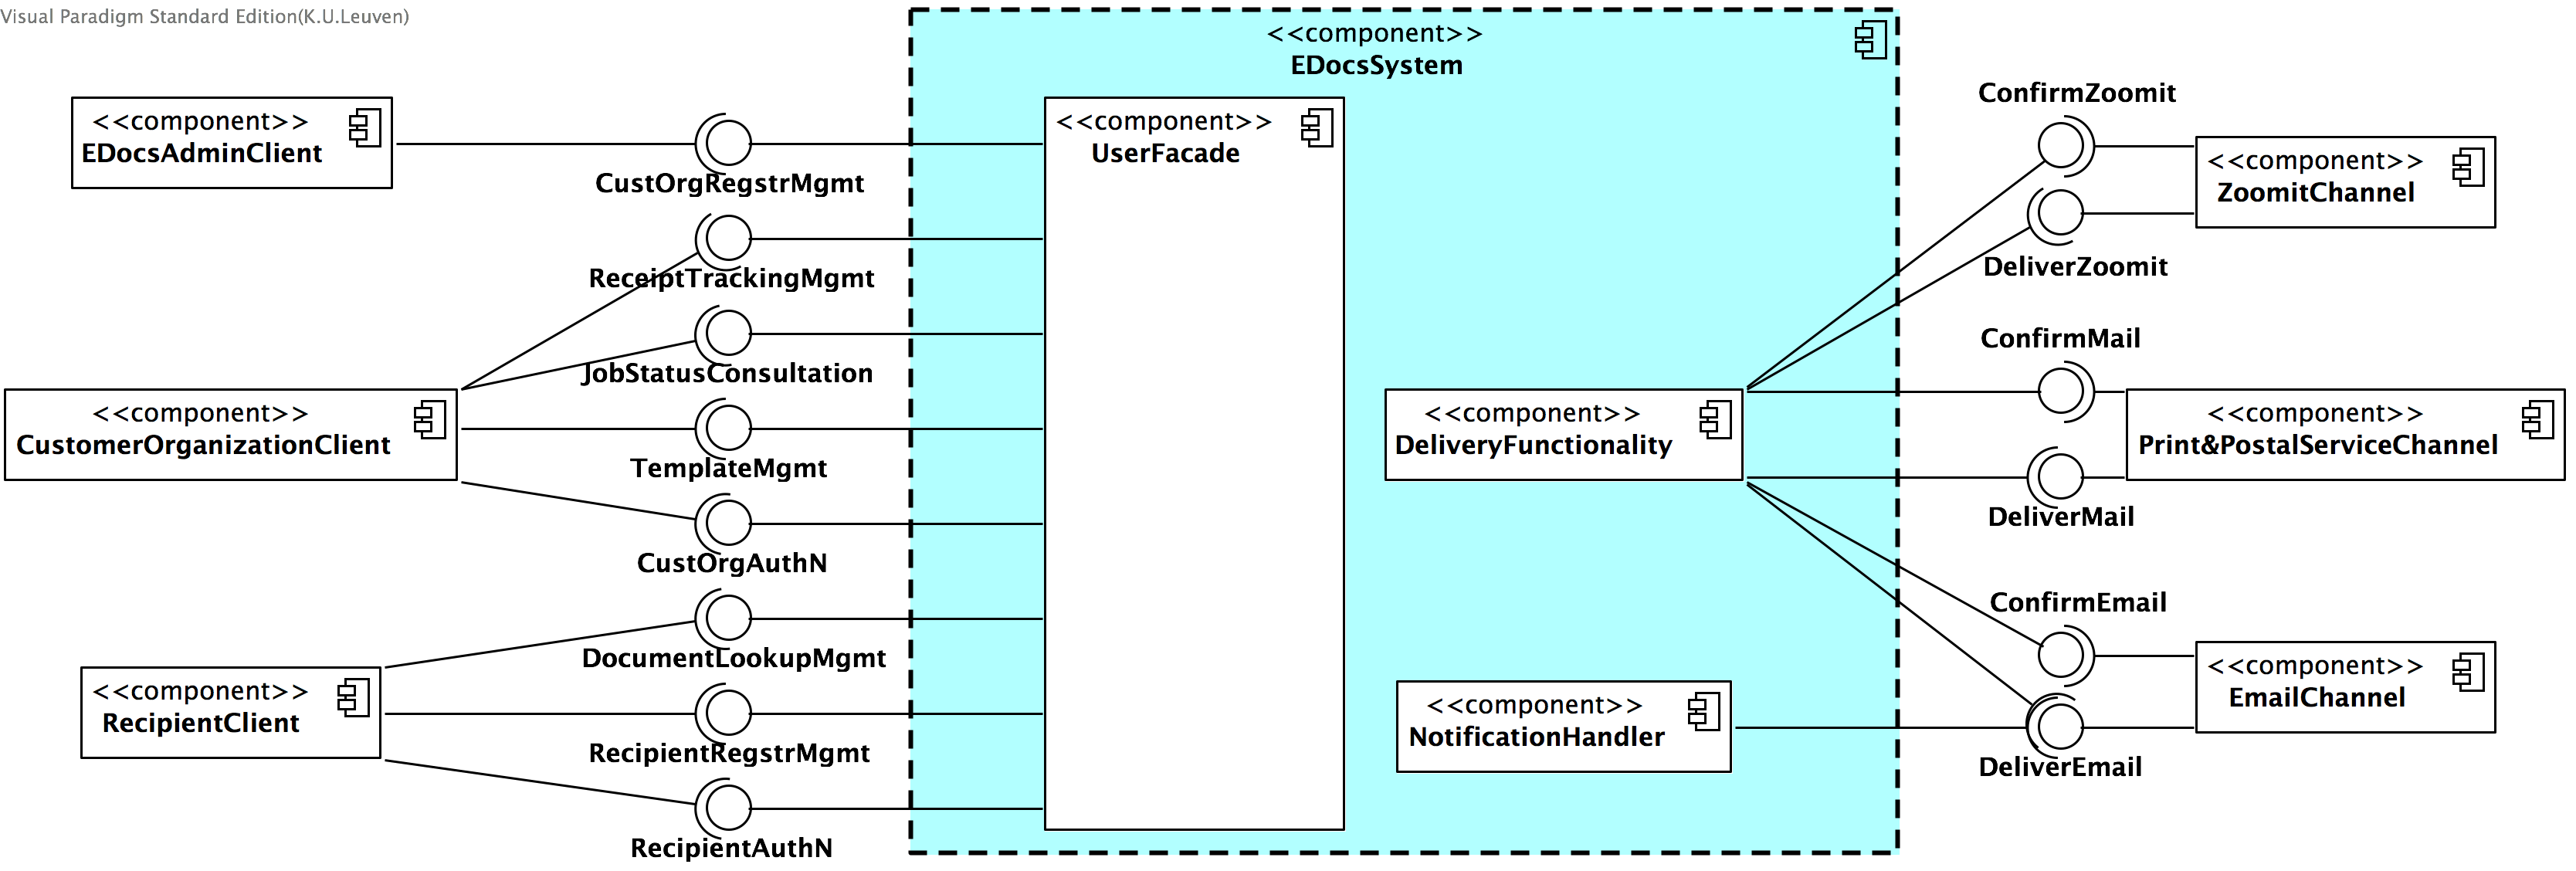
\includegraphics[width=0.8\textwidth]{ContextDiagram.png}
	\caption{Context diagram for the client-server view.}
	\label{fig:cc-context}
\end{figure}

The primary diagram and accompanying explanation.

\begin{figure}[!htp]
	\centering
	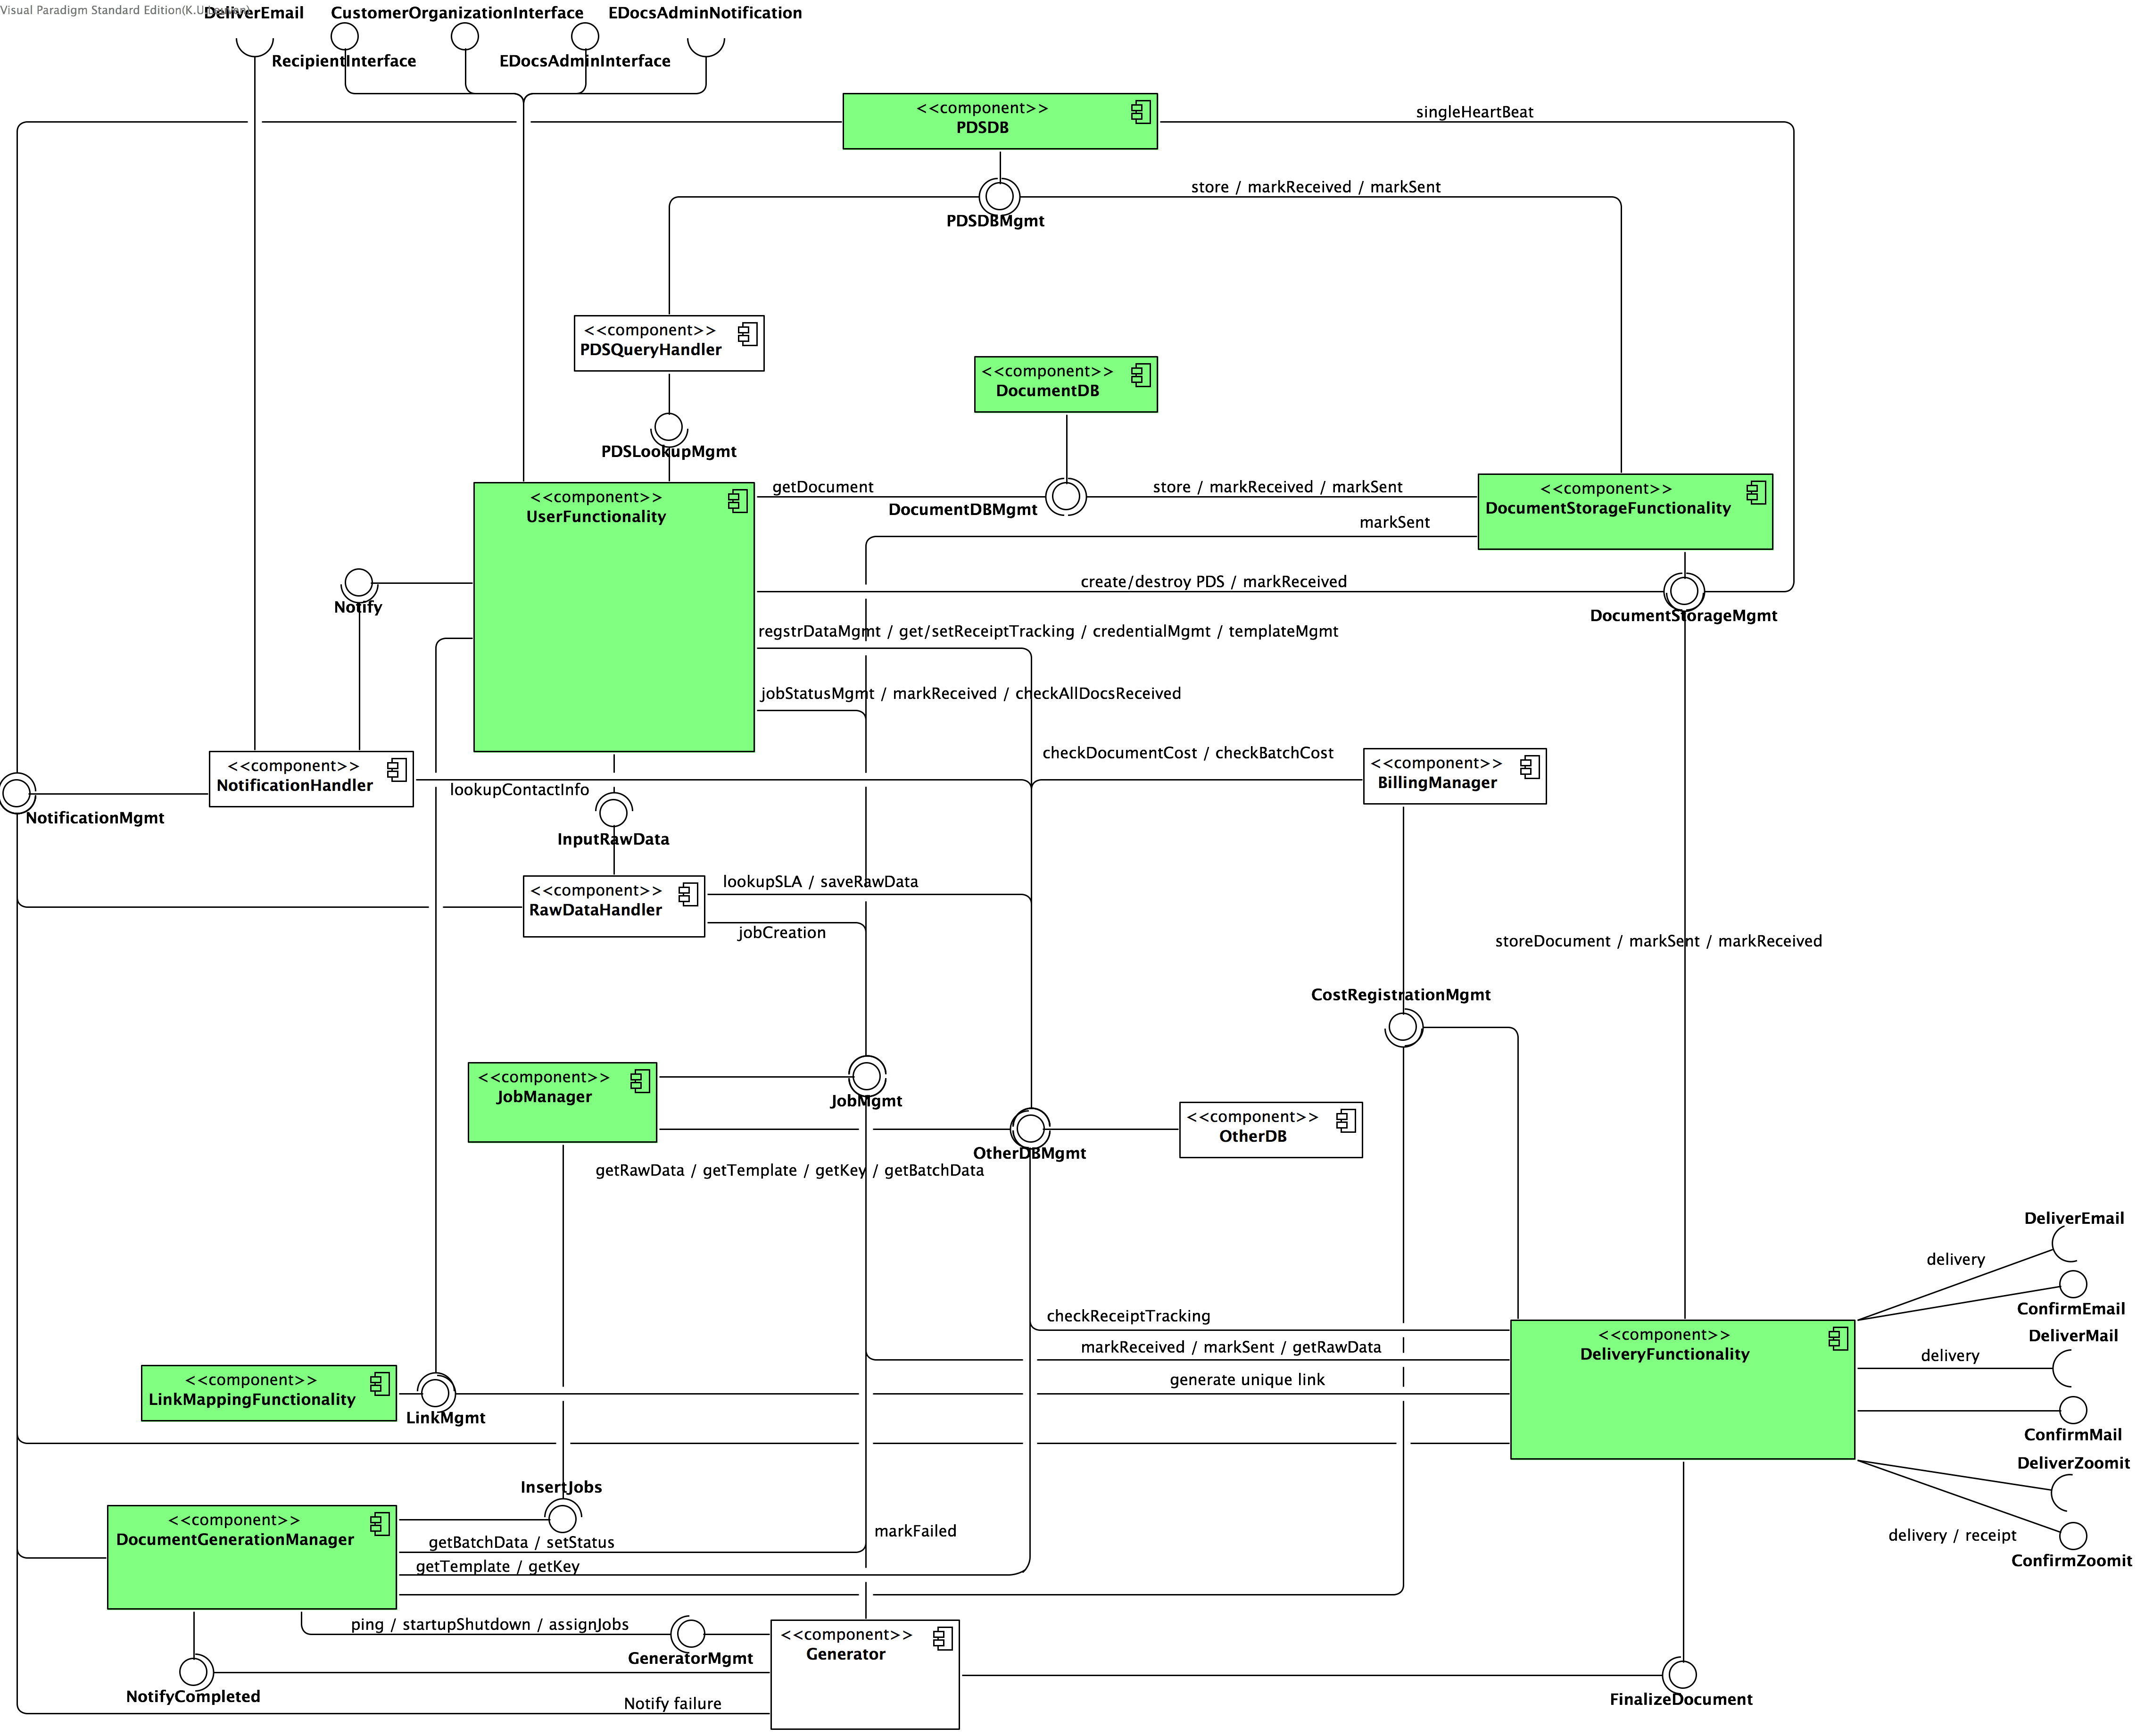
\includegraphics[width=0.8\textwidth]{ClientServerView.png}
	\caption{Primary diagram of the client-server view.}
	\label{fig:cs-primary}
\end{figure}

\subsection{Main architectural decisions}
Discuss your architectural decisions for the most important requirements in
more detail using the components of the client-server view.
Pay attention to the solutions that you employed and the alternatives that you
considered.
The explanation here must be self-contained and complete.
Imagine you had to describe how the architecture supports the core
functionality to someone that is looking at the client-server view only.
Hide unnecessary details (these should be shown in the decomposition view).

\subsubsection{ReqX\@: requirement name}
Describe the design choices related to \emph{ReqX} together with the rationale
of why these choices where made.

\subsubsection*{Alternatives considered}
\paragraph{Alternative(s) for choice 1} Explain what alternative(s) you
considered for this design choice and why they where not selected.

\section{Decomposition view (UML Component diagram)}\label{sec:decomposition}
Discuss the decompositions of the components of the client-server view which
you have further decomposed.

\subsection{ComponentX}
\begin{figure}[!htp]
    \centering
    %\includegraphics[width=\textwidth]{}
    \missingfigure[figwidth=0.8\textwidth]{Diagram showing decomposition of
        ComponentX}
    \caption{Decomposition of \texttt{ComponentX}}\label{fig:decomp-componentx}
\end{figure}

Describe the decomposition of \texttt{ComponentX} and how this relates to the
requirements.

\section{Deployment view (UML Deployment diagram)}\label{sec:deployment}
Describe the context diagram for the deployment view.
For example, which protocols are used for communication with external systems
and why?

\begin{figure}[!htp]
    \centering
    %\includegraphics[width=\textwidth]{}
    \missingfigure[figwidth=0.8\textwidth]{Context diagram for the deployment
        view.}
    \caption{Context diagram for the deployment view.}\label{fig:depl_context}
\end{figure}

The primary deployment diagram itself and accompanying explanation.
Pay attention to the parts of the deployment diagram which are crucial for
achieving certain non-functional requirements.
Also discuss any alternative deployments that you considered.

\begin{figure}[!htp]
    \centering
    %\includegraphics[width=\textwidth]{}
    \missingfigure[figwidth=0.8\textwidth]{Primary diagram for the deployment
        view.}
    \caption{Primary diagram for the deployment view.}\label{fig:depl_primary}
\end{figure}

\section{Scenarios}\label{sec:scenarios}
Illustrate how your architecture fulfills the most important data flows.
As a rule of thumb, focus on the scenario of the domain description.
Describe the scenario in terms of architectural components using UML Sequence
diagrams and further explain the most important interactions in text.
Illustrating the scenarios serves as a quick validation of the completeness of
your architecture.
If you notice at this point that for some reason, certain functionality or
qualities are not addressed sufficiently in your architecture, it suffices to
document this, together with a rationale of why this is the case according to
you.
You do not have to further refine you architecture at this point.

\subsection{Scenario 1}
Shortly describe the scenario shown in this subsection.
Show the complete scenario using one or more sequence diagrams.

\begin{figure}[!htp]
    \centering
    %\includegraphics[width=\textwidth]{}
    \missingfigure[figwidth=0.8\textwidth]{Sequence diagram scenario 1}
    \caption{The system behavior for the first scenario.
        }\label{fig:seq_scenario1}
\end{figure}

\appendix
\section{Element catalog}\label{app:catalog}
List all components and describe their responsibilities and provided
interfaces.
Per interface, list all methods using a Java-like syntax and describe their
effect and exceptions if any.
List all elements and interfaces alphabetically for ease of navigation.





\subsection{Component 1}
\begin{itemize}
    \item \textbf{Description:} Responsibilities of the component.
    \item \textbf{Super-component:} The direct super-component, if any.
    \item \textbf{Sub-components:} the direct sub-components, if any.
\end{itemize}

\subsubsection*{Provided interfaces}
\begin{itemize}
    \item InterfaceA
    \begin{itemize}
        \item \texttt{returntType1 operation1(ParamType param) throws SomeException}
        \begin{itemize}
            \item Effect: Describe the effect of the operation
            \item Exceptions:
            \begin{itemize}
                \item SomeException: Describe when the exception is thrown.
            \end{itemize}

            \item \texttt{void operation2(ParamType2 param)}
            \begin{itemize}
                \item Effect: Describe the effect of the operation
                \item Exceptions: None
            \end{itemize}
        \end{itemize}
    \end{itemize}

    \item InterfaceB
    \begin{itemize}
        \item \texttt{returntType2 operation3()}
        \begin{itemize}
            \item Effect: Describe the effect of the operation
            \item Exceptions: None
        \end{itemize}
    \end{itemize}
\end{itemize}


\subsection{AuthenticationHandler}
\begin{itemize}
    \item \textbf{Description:} The \texttt{AuthenticationHandler} is responsible for authenticating Registered recipients and Customer organizations. The architecture does not specify the means of authentication (e.g. the type of credentials). The credentials are stored in the \texttt{UserDB}.
    \item \textbf{Super-component:} \texttt{UserFacade}
    \item \textbf{Sub-components:} None
\end{itemize}

\subsubsection*{Provided interfaces}
\begin{itemize}
    \item AuthN
    \begin{itemize}
        \item \texttt{RecipientId getRecipientId(SessionId sessionId) throws NoSuchSessionException}
        \begin{itemize}
            \item Effect: The \texttt{AuthenticationHandler} fetches and returns the Registered Recipient's identifier corresponding to the \texttt{sessionId} from the \texttt{sessionDB}.
            \item Exceptions:
            \begin{itemize}
                \item NoSuchSessionException: Thrown if no session exists with the given identifiers, or if the session belongs to a customer organization.
            \end{itemize}
		\end{itemize}
		
        \item \texttt{CustomerId getCustomerId(SessionId sessionId) throws NoSuchSessionException}
        \begin{itemize}
             \item Effect: The \texttt{AuthenticationHandler} fetches and returns the Customer Organization's identifier corresponding to the \texttt{sessionId} from the \texttt{sessionDB}.
             \item Exceptions:
             \begin{itemize}
                \item NoSuchSessionException: Thrown if no session exists with the given identifier, or if the session belongs to a registered recipient.
             \end{itemize}
        \end{itemize}
        
        \item \texttt{Boolean logout(SessionId sessionId)}
        \begin{itemize}
            \item Effect: The \texttt{AuthenticationHandler} will remove the session with the given id from the \texttt{SessionDB}. If no such session exists, nothing is changed and no exception is thrown.
            \item Exceptions: None
        \end{itemize}
        
        \item \texttt{SessionId login(Credentials credentials) throws InvalidCredentialsException}
        \begin{itemize}
            \item Effect: The \texttt{AuthenticationHandler} verifies the \texttt{credentials} using the \texttt{UserDB}. If they are correct, the \texttt{AuthenticationHandler} creates a new session using the \texttt{SessionDB}, stores the id of the user (i.e. the Registered Recipient id or Customer Organization id) as an attribute in this session and returns the id of the new session. The id of the user is present in the given credentials.
            \item Exceptions: 
            \begin{itemize}
                \item InvalidCredentialsException: Thrown if the given credentials are invalid.
             \end{itemize}
        \end{itemize}
    \end{itemize}
    
    
	\item CheckSession
    \begin{itemize}
        \item \texttt{Map<SessionAttributeKey, SessionAttributeValue> verifySession(SessionId sesionId) throws NoSuchsSessionException}
        \begin{itemize}
            \item Effect: The \texttt{AuthenticationHandler} verifies whether a session with the given id exists in the \texttt{SessionDB} and if so, returns all its associated attributes.
            \item Exceptions:
            \begin{itemize}
                \item NoSuchSessionException: Thrown if no session exists with the given identifiers.
             \end{itemize}
        \end{itemize}
    \end{itemize}	
\end{itemize}

\subsection{BillingManager}
\begin{itemize}
    \item \textbf{Description:} Responsibilities of the component.
    \item \textbf{Super-component:} The direct super-component, if any.
    \item \textbf{Sub-components:} the direct sub-components, if any.
\end{itemize}

\subsubsection*{Provided interfaces}
\begin{itemize}
    \item InterfaceA
    \begin{itemize}
        \item \texttt{returntType1 operation1(ParamType param) throws SomeException}
        \begin{itemize}
            \item Effect: Describe the effect of the operation
            \item Exceptions:
            \begin{itemize}
                \item SomeException: Describe when the exception is thrown.
            \end{itemize}

            \item \texttt{void operation2(ParamType2 param)}
            \begin{itemize}
                \item Effect: Describe the effect of the operation
                \item Exceptions: None
            \end{itemize}
        \end{itemize}
    \end{itemize}

    \item InterfaceB
    \begin{itemize}
        \item \texttt{returntType2 operation3()}
        \begin{itemize}
            \item Effect: Describe the effect of the operation
            \item Exceptions: None
        \end{itemize}
    \end{itemize}
\end{itemize}

\subsection{CustomerOrganizationFacade}
\begin{itemize}
    \item \textbf{Description:} Responsibilities of the component.
    \item \textbf{Super-component:} The direct super-component, if any.
    \item \textbf{Sub-components:} the direct sub-components, if any.
\end{itemize}

\subsubsection*{Provided interfaces}
\begin{itemize}
    \item InterfaceA
    \begin{itemize}
        \item \texttt{returntType1 operation1(ParamType param) throws SomeException}
        \begin{itemize}
            \item Effect: Describe the effect of the operation
            \item Exceptions:
            \begin{itemize}
                \item SomeException: Describe when the exception is thrown.
            \end{itemize}

            \item \texttt{void operation2(ParamType2 param)}
            \begin{itemize}
                \item Effect: Describe the effect of the operation
                \item Exceptions: None
            \end{itemize}
        \end{itemize}
    \end{itemize}

    \item InterfaceB
    \begin{itemize}
        \item \texttt{returntType2 operation3()}
        \begin{itemize}
            \item Effect: Describe the effect of the operation
            \item Exceptions: None
        \end{itemize}
    \end{itemize}
\end{itemize}


\subsection{Completer}
\begin{itemize}
    \item \textbf{Description:} The \texttt{Completer} is responsible for fetching the raw data an applicable meta-data for a group of \texttt{JobIds} when a \texttt{Generator} instance requires a new group of jobs.
    \item \textbf{Super-component:} \texttt{DocumentGenerationManager}
    \item \textbf{Sub-components:} None
\end{itemize}

\subsubsection*{Provided interfaces}
\begin{itemize}
    \item Complete
    \begin{itemize}
        \item \texttt{CompletePartialBatchData getComplete(BatchId batchId, List<JobId> jobIds )}
        \begin{itemize}
            \item Effect: The \texttt{Completer} fetches data needed by a \texttt{Generator} for generation of the documents corrseponding to the\texttt{JobIds} belonging to the same batch, which is identified by \texttt{BatchId}.
            \item Exceptions: None
        \end{itemize}
    \end{itemize}
\end{itemize}

\subsection{DB}
\begin{itemize}
    \item \textbf{Description:} Responsibilities of the component.
    \item \textbf{Super-component:} The direct super-component, if any.
    \item \textbf{Sub-components:} the direct sub-components, if any.
\end{itemize}

\subsubsection*{Provided interfaces}
\begin{itemize}
    \item InterfaceA
    \begin{itemize}
        \item \texttt{returntType1 operation1(ParamType param) throws SomeException}
        \begin{itemize}
            \item Effect: Describe the effect of the operation
            \item Exceptions:
            \begin{itemize}
                \item SomeException: Describe when the exception is thrown.
            \end{itemize}

            \item \texttt{void operation2(ParamType2 param)}
            \begin{itemize}
                \item Effect: Describe the effect of the operation
                \item Exceptions: None
            \end{itemize}
        \end{itemize}
    \end{itemize}

    \item InterfaceB
    \begin{itemize}
        \item \texttt{returntType2 operation3()}
        \begin{itemize}
            \item Effect: Describe the effect of the operation
            \item Exceptions: None
        \end{itemize}
    \end{itemize}
\end{itemize}

\subsection{DocumentDB}
\begin{itemize}
    \item \textbf{Description:} Responsibilities of the component.
    \item \textbf{Super-component:} The direct super-component, if any.
    \item \textbf{Sub-components:} the direct sub-components, if any.
\end{itemize}

\subsubsection*{Provided interfaces}
\begin{itemize}
    \item InterfaceA
    \begin{itemize}
        \item \texttt{returntType1 operation1(ParamType param) throws SomeException}
        \begin{itemize}
            \item Effect: Describe the effect of the operation
            \item Exceptions:
            \begin{itemize}
                \item SomeException: Describe when the exception is thrown.
            \end{itemize}

            \item \texttt{void operation2(ParamType2 param)}
            \begin{itemize}
                \item Effect: Describe the effect of the operation
                \item Exceptions: None
            \end{itemize}
        \end{itemize}
    \end{itemize}

    \item InterfaceB
    \begin{itemize}
        \item \texttt{returntType2 operation3()}
        \begin{itemize}
            \item Effect: Describe the effect of the operation
            \item Exceptions: None
        \end{itemize}
    \end{itemize}
\end{itemize}

\subsection{CustOrgRegistrationManager}
\begin{itemize}
    \item \textbf{Description:} Responsibilities of the component.
    \item \textbf{Super-component:} The direct super-component, if any.
    \item \textbf{Sub-components:} the direct sub-components, if any.
\end{itemize}

\subsubsection*{Provided interfaces}
\begin{itemize}
    \item InterfaceA
    \begin{itemize}
        \item \texttt{returntType1 operation1(ParamType param) throws SomeException}
        \begin{itemize}
            \item Effect: Describe the effect of the operation
            \item Exceptions:
            \begin{itemize}
                \item SomeException: Describe when the exception is thrown.
            \end{itemize}

            \item \texttt{void operation2(ParamType2 param)}
            \begin{itemize}
                \item Effect: Describe the effect of the operation
                \item Exceptions: None
            \end{itemize}
        \end{itemize}
    \end{itemize}

    \item InterfaceB
    \begin{itemize}
        \item \texttt{returntType2 operation3()}
        \begin{itemize}
            \item Effect: Describe the effect of the operation
            \item Exceptions: None
        \end{itemize}
    \end{itemize}
\end{itemize}

\subsection{DocumentGenerationManager}
\begin{itemize}
    \item \textbf{Description:} The \texttt{DocumentGenerationManager} monitors the availability of the \texttt{Generator} components using the Ping interface. The \texttt{DocumentGenerationManager} keeps track of the jobs assigned to and being processed by the \texttt{Generators}. To minimize the overhead of the job coordination, the \texttt{DocumentGenerationManager} assigns jobs to the \texttt{Generators} in groups of more than one job that are part of the same batch. If a \texttt{Generator} fails to complete its jobs, the \texttt{DocumentGenerationManager} can restart these failed jobs. \\ It prioritizes jobs based on thei deadlines ansd schedules them according to \emph{P1}.
    \item \textbf{Super-component:} None
    \item \textbf{Sub-components:} \texttt{Completer}, \texttt{GenerationManager}, \texttt{KeyCache}, \texttt{Scheduler}, \texttt{TemplateCache}
\end{itemize}

\subsubsection*{Provided interfaces}
\begin{itemize}
    \item InsertJobs
    \begin{itemize}
        \item \texttt{returntType1 operation1(ParamType param) throws SomeException}
        \begin{itemize}
            \item Effect: Describe the effect of the operation
            \item Exceptions:
            \begin{itemize}
                \item SomeException: Describe when the exception is thrown.
            \end{itemize}

            \item \texttt{void operation2(ParamType2 param)}
            \begin{itemize}
                \item Effect: Describe the effect of the operation
                \item Exceptions: None
            \end{itemize}
        \end{itemize}
    \end{itemize}

    \item NotifyCompleted
    \begin{itemize}
        \item \texttt{void notifyCompletedAndGiveMeMore(GeneratorId id)}
        \begin{itemize}
            \item Effect: The \texttt{DocumentGenerationManager} gets notified that the document processing jobs assigned to the \texttt{Generator} identified by an \texttt{id} are completed. 
            %It looks up the \texttt{JobIds} of the jobs assigned to the \texttt{Generator}. It notifies the \texttt{Scheduler} that the job
            \item Exceptions: None
        \end{itemize}
        
        \item \texttt{void notifyCompletedAndIAmShuttingDown(GeneratorId id)}
            \begin{itemize}
                \item Effect: The \texttt{DocumentGenerationManager} gets notified that the document processing jobs assigned to the \texttt{Generator} identified by an \texttt{id} are completed. 
                \item Exceptions: None
            \end{itemize}
        \end{itemize}
    \end{itemize}

\subsection{DocumentStorageManager}
\begin{itemize}
    \item \textbf{Description:} Responsibilities of the component.
    \item \textbf{Super-component:} The direct super-component, if any.
    \item \textbf{Sub-components:} the direct sub-components, if any.
\end{itemize}

\subsubsection*{Provided interfaces}
\begin{itemize}
    \item InterfaceA
    \begin{itemize}
        \item \texttt{returntType1 operation1(ParamType param) throws SomeException}
        \begin{itemize}
            \item Effect: Describe the effect of the operation
            \item Exceptions:
            \begin{itemize}
                \item SomeException: Describe when the exception is thrown.
            \end{itemize}

            \item \texttt{void operation2(ParamType2 param)}
            \begin{itemize}
                \item Effect: Describe the effect of the operation
                \item Exceptions: None
            \end{itemize}
        \end{itemize}
    \end{itemize}

    \item InterfaceB
    \begin{itemize}
        \item \texttt{returntType2 operation3()}
        \begin{itemize}
            \item Effect: Describe the effect of the operation
            \item Exceptions: None
        \end{itemize}
    \end{itemize}
\end{itemize}

\subsection{DeliveryFunctionality}
\begin{itemize}
    \item \textbf{Description:} Responsibilities of the component.
    \item \textbf{Super-component:} The direct super-component, if any.
    \item \textbf{Sub-components:} the direct sub-components, if any.
\end{itemize}

\subsubsection*{Provided interfaces}
\begin{itemize}
    \item InterfaceA
    \begin{itemize}
        \item \texttt{returntType1 operation1(ParamType param) throws SomeException}
        \begin{itemize}
            \item Effect: Describe the effect of the operation
            \item Exceptions:
            \begin{itemize}
                \item SomeException: Describe when the exception is thrown.
            \end{itemize}

            \item \texttt{void operation2(ParamType2 param)}
            \begin{itemize}
                \item Effect: Describe the effect of the operation
                \item Exceptions: None
            \end{itemize}
        \end{itemize}
    \end{itemize}

    \item InterfaceB
    \begin{itemize}
        \item \texttt{returntType2 operation3()}
        \begin{itemize}
            \item Effect: Describe the effect of the operation
            \item Exceptions: None
        \end{itemize}
    \end{itemize}
\end{itemize}

\subsection{EDocsFacade}
\begin{itemize}
    \item \textbf{Description:} Responsibilities of the component.
    \item \textbf{Super-component:} The direct super-component, if any.
    \item \textbf{Sub-components:} the direct sub-components, if any.
\end{itemize}

\subsubsection*{Provided interfaces}
\begin{itemize}
    \item InterfaceA
    \begin{itemize}
        \item \texttt{returntType1 operation1(ParamType param) throws SomeException}
        \begin{itemize}
            \item Effect: Describe the effect of the operation
            \item Exceptions:
            \begin{itemize}
                \item SomeException: Describe when the exception is thrown.
            \end{itemize}

            \item \texttt{void operation2(ParamType2 param)}
            \begin{itemize}
                \item Effect: Describe the effect of the operation
                \item Exceptions: None
            \end{itemize}
        \end{itemize}
    \end{itemize}

    \item InterfaceB
    \begin{itemize}
        \item \texttt{returntType2 operation3()}
        \begin{itemize}
            \item Effect: Describe the effect of the operation
            \item Exceptions: None
        \end{itemize}
    \end{itemize}
\end{itemize}

\subsection{EmailFacade}
\begin{itemize}
    \item \textbf{Description:} The \texttt{EmailFacade} is responsible for sending documents to  Unregistered by e-mail when receipt tracking is turned off. When receipt tracking is turned on for an Unregistered Recipient, it sends an e-mail containing a short description of the received document
    \item \textbf{Super-component:} \texttt{DeliveryFunctionality}
    \item \textbf{Sub-components:} None
\end{itemize}

\subsubsection*{Provided interfaces}
\begin{itemize}
    \item InterfaceA
    \begin{itemize}
        \item \texttt{returntType1 operation1(ParamType param) throws SomeException}
        \begin{itemize}
            \item Effect: Describe the effect of the operation
            \item Exceptions:
            \begin{itemize}
                \item SomeException: Describe when the exception is thrown.
            \end{itemize}

            \item \texttt{void operation2(ParamType2 param)}
            \begin{itemize}
                \item Effect: Describe the effect of the operation
                \item Exceptions: None
            \end{itemize}
        \end{itemize}
    \end{itemize}

    \item InterfaceB
    \begin{itemize}
        \item \texttt{returntType2 operation3()}
        \begin{itemize}
            \item Effect: Describe the effect of the operation
            \item Exceptions: None
        \end{itemize}
    \end{itemize}
\end{itemize}

\subsection{Generator}
\begin{itemize}
    \item \textbf{Description:} A \texttt{Generator} generates the documents and forwards them to \texttt{OtherFunctionality} to store and deliver them. Its availability is monitored by the \texttt{DocumenGenerationManager} with the Ping interface. A \texttt{Generator} is also responsible of notifying the \texttt{OtherFunctionality} that it does not have all of the data required to fill in the template.
    \item \textbf{Super-component:} None
    \item \textbf{Sub-components:} None
\end{itemize}

\subsubsection*{Provided interfaces}
\begin{itemize}
    \item AssignJobs
    \begin{itemize}
        \item \texttt{void assignJobs(CompletePartialBatchData batchData)}
        \begin{itemize}
            \item Effect: Describe the effect of the operation
            \item Exceptions:
            \begin{itemize}
                \item SomeException: Describe when the exception is thrown.
            \end{itemize}

            \item \texttt{void operation2(ParamType2 param)}
            \begin{itemize}
                \item Effect: Describe the effect of the operation
                \item Exceptions: None
            \end{itemize}
        \end{itemize}
    \end{itemize}

    \item Startup/ShutDown
    \begin{itemize}
        \item \texttt{void startUp(GeneratorId generatorId)}
        \begin{itemize}
            \item Effect: Starts up the \texttt{Generator} instance an gives it the given \texttt{GeneratorId}. 
            \item Exceptions: None
        \end{itemize}
          \item \texttt{void shutDown()}
        \begin{itemize}
            \item Effect: The \texttt{Generator} completes its assigned group of document generation jobs and report back completion to the \texttt{DocumentGenerationManager}, after which is shuts down.
            \item Exceptions: None
        \end{itemize}
    \end{itemize}
    
    \item Ping
    \begin{itemize}
        \item \texttt{Echo ping()}
        \begin{itemize}
            \item Effect: The \texttt{Generator} will respond to the ping request by sending an echo response. This is used by the \texttt{GeneratorManager} to check whether the \texttt{Generator} is available.
            \item Exceptions: None
        \end{itemize}
    \end{itemize}
\end{itemize}
\subsection{GeneratorManager}
\begin{itemize}
    \item \textbf{Description:} The \texttt{GenerationManager} is responsible for monitoring the \texttt{Generator} instances. It starts up or shuts down these instances based on the number of required instances indicated by the \texttt{Scheduler}.
    \item \textbf{Super-component:}  \texttt{DocumentGenerationManager}
    \item \textbf{Sub-components:} None
\end{itemize}

\subsubsection*{Provided interfaces}
\begin{itemize}
    \item NotifyCompleted
    \begin{itemize}
        \item \texttt{void notifyCompletedAndGiveMeMore(GeneratorId id)}
        \begin{itemize}
            \item Effect: The \texttt{DocumentGenerationManager} gets notified that the document processing jobs assigned to the \texttt{Generator} identified by an \texttt{id} are completed. 
            %It looks up the \texttt{JobIds} of the jobs assigned to the \texttt{Generator}. It notifies the \texttt{Scheduler} that the job
            \item Exceptions: None
        \end{itemize}
    \end{itemize}
\end{itemize}

\subsection{JobFacade}
\begin{itemize}
    \item \textbf{Description:} Responsibilities of the component.
    \item \textbf{Super-component:} The direct super-component, if any.
    \item \textbf{Sub-components:} the direct sub-components, if any.
\end{itemize}

\subsubsection*{Provided interfaces}
\begin{itemize}
    \item InterfaceA
    \begin{itemize}
        \item \texttt{returntType1 operation1(ParamType param) throws SomeException}
        \begin{itemize}
            \item Effect: Describe the effect of the operation
            \item Exceptions:
            \begin{itemize}
                \item SomeException: Describe when the exception is thrown.
            \end{itemize}

            \item \texttt{void operation2(ParamType2 param)}
            \begin{itemize}
                \item Effect: Describe the effect of the operation
                \item Exceptions: None
            \end{itemize}
        \end{itemize}
    \end{itemize}

    \item InterfaceB
    \begin{itemize}
        \item \texttt{returntType2 operation3()}
        \begin{itemize}
            \item Effect: Describe the effect of the operation
            \item Exceptions: None
        \end{itemize}
    \end{itemize}
\end{itemize}

\subsection{KeyCache}
\begin{itemize}
    \item \textbf{Description:} The \texttt{KeyCache} caches the keys which are most recently used for document generation. The \texttt{Completer} has to fetch a key every time a \texttt{Generator} instance requests new jobs, while the key will be the same for all jobs belonging to the same batch. The \texttt{KeyCache} avoids that the key storage system becomes a bottleneck for document generations. The keys are cached based on the \texttt{CustomerId} of a Customer Organization.
    \item \textbf{Super-component:}  \texttt{DocumentGenerationManager}.
    \item \textbf{Sub-components:} None
\end{itemize}

\subsubsection*{Provided interfaces}
\begin{itemize}
    \item GetKey
    \begin{itemize}
        \item \texttt{Key getKey(CustomerId customerId) throws NoSuchKeyException}
        \begin{itemize}
            \item Effect: The \texttt{KeyCache} looks into its cache for the \texttt{Key} belonging to the customer organisation with id \texttt{customerId}. If the \texttt{Key} is in its cache, it returns it. If the \texttt{Key} is not in its cache, it asks \texttt{OtherFunctionality} for the \texttt{Key} and stores it in its cache, after which it returns that \texttt{Key}.
            \item Exceptions:
            \begin{itemize}
                \item NoSuchKeyException: Thrown if there is no key for the given \texttt{customerId}.
            \end{itemize}
        \end{itemize}
    \end{itemize}
\end{itemize}

\subsection{LinkManager}
\begin{itemize}
    \item \textbf{Description:} Responsibilities of the component.
    \item \textbf{Super-component:} The direct super-component, if any.
    \item \textbf{Sub-components:} the direct sub-components, if any.
\end{itemize}

\subsubsection*{Provided interfaces}
\begin{itemize}
    \item InterfaceA
    \begin{itemize}
        \item \texttt{returntType1 operation1(ParamType param) throws SomeException}
        \begin{itemize}
            \item Effect: Describe the effect of the operation
            \item Exceptions:
            \begin{itemize}
                \item SomeException: Describe when the exception is thrown.
            \end{itemize}

            \item \texttt{void operation2(ParamType2 param)}
            \begin{itemize}
                \item Effect: Describe the effect of the operation
                \item Exceptions: None
            \end{itemize}
        \end{itemize}
    \end{itemize}

    \item InterfaceB
    \begin{itemize}
        \item \texttt{returntType2 operation3()}
        \begin{itemize}
            \item Effect: Describe the effect of the operation
            \item Exceptions: None
        \end{itemize}
    \end{itemize}
\end{itemize}

\subsection{PDSDB}
\begin{itemize}
    \item \textbf{Description:} The \texttt{PDSDB} component is responsible for storing the database of documents in the personal document stores.  That database is separated from all other persistent data so that its failure \emph{``does not affect the availability of other types of persistent data''}, as required by \emph{Av2}.
    \item \textbf{Super-component:} None
    \item \textbf{Sub-components:} \texttt{PDSDBReplica}, \texttt{PDSLongTermDocumentManager}, \texttt{PDSReplicationManager}
\end{itemize}

\subsubsection*{Provided interfaces}
\begin{itemize}
    \item DocumentMgmt
    \begin{itemize}
        \item \texttt{Tuple<Document, MetaData> getDocument(DocumentId id)}
        \begin{itemize}
            \item Effect: The \texttt{PDSDB} will fetch and return the document corresponding to \texttt{DocumentId} id.
            \item Exceptions: None
         \end{itemize}
         
         \item \texttt{List<Document> getAllDocumentMetaDataOf(RecipientId recipientId)}
        \begin{itemize}
            \item Effect: The \texttt{PDSDB} will fetch and return all the meta-data of the documents belonging to the Registered Recipient identified by \texttt{recipientId}.
            \item Exceptions: None
         \end{itemize}   
% MERK OP: in het sequence diagram geeft dit een zeer geke return waarde terug: OK
		\item \texttt{void storeDocument(DocumentId id, Document doc, DocumentMetaData md)}
        \begin{itemize}
            \item Effect: The \texttt{PDSDB} will store the given document\texttt{doc} together with the provided meta-data \texttt{md}.
            \item Exceptions:  None 
        \end{itemize}
         
         \item \texttt{void storeDocuments(List<Tuple<DocumentId, Document, DocumentMetaData>> documentList)}
         \begin{itemize}
                \item Effect: Describe the effect of the operation
                \item Exceptions: None
         \end{itemize}
    \end{itemize}
\end{itemize}

\subsection{PDSDBReplica}
\begin{itemize}
    \item \textbf{Description:} The \texttt{PDSDBReplica} is responsible for actually storing the documents.
    \item \textbf{Super-component:} \texttt{PDSDB}
    \item \textbf{Sub-components:} None
\end{itemize}

\subsubsection*{Provided interfaces}
\begin{itemize}
    \item ExtendedDocumentMgmt
    \begin{itemize}
    % MERK OP: mogelijk is het meer dan een lijst van documenten die over gedragen moet worden. Er staat een goed voorbeeld in de PMS
    	\item \texttt{List<Document> getAllDocumentsOf(TimeStamp whenFailed)}
        \begin{itemize}
            \item Effect: Describe the effect of the operation
            \item Exceptions:
            \begin{itemize}
                \item SomeException: Describe when the exception is thrown.
            \end{itemize}
        \end{itemize}    
            
        \item \texttt{List<Document> getDocumentsSince(TimeStamp whenFailed)}
        \begin{itemize}
            \item Effect: Describe the effect of the operation
            \item Exceptions:
            \begin{itemize}
                \item SomeException: Describe when the exception is thrown.
            \end{itemize}
         \end{itemize}   
% MERK OP: in het sequence diagram geeft dit een zeer geke return waarde terug: OK
         \item \texttt{void storeDocuments(List<Tuple<DocumentId, Document, DocumentMetaData>> documentList)}
         \begin{itemize}
            \item Effect: Describe the effect of the operation
            \item Exceptions: None
         \end{itemize}
		 \item \texttt{void storeDocument(DocumentId documentId, Document document, DocumentMetaDate documentMetaData)}
         \begin{itemize}
            \item Effect: The \texttt{PDSDBReplica} stores the given document with its \\texttt{DocumentId} and meta-data.
            \item Exceptions: None
         \end{itemize}            
    \end{itemize}
    
    \begin{itemize}
        \item \texttt{Tuple<Document, MetaData> getDocument(DocumentId id)}
        \begin{itemize}
            \item Effect: The \texttt{PDSDB} will fetch and return the document corresponding to \texttt{DocumentId} id.
            \item Exceptions: None
         \end{itemize}
         
         \item \texttt{List<Document> getAllDocumentMetaDataOf(RecipientId recipientId)}
        \begin{itemize}
            \item Effect: The \texttt{PDSDB} will fetch and return all the meta-data of the documents belonging to the Registered Recipient identified by \texttt{recipientId}.
            \item Exceptions: None
         \end{itemize}   
% MERK OP: in het sequence diagram geeft dit een zeer geke return waarde terug: OK
		\item \texttt{void storeDocument(DocumentId id, Document doc, DocumentMetaData md)}
        \begin{itemize}
            \item Effect: The \texttt{PDSDB} will store the given document\texttt{doc} together with the provided meta-data \texttt{md}.
            \item Exceptions:  None 
        \end{itemize}
         
         \item \texttt{void storeDocuments(List<Tuple<DocumentId, Document, DocumentMetaData>> documentList)}
         \begin{itemize}
                \item Effect: Describe the effect of the operation
                \item Exceptions: None
         \end{itemize}
    \end{itemize}
    
    \item Ping
    \begin{itemize}
        \item \texttt{Echo ping()}
        \begin{itemize}
            \item Effect: The \texttt{PDSDBReplica} will respond to the ping request by sending an echo response. This is used by the \texttt{PDSReplicationManager} to check whether the \texttt{PDSDBReplica} is available.
            \item Exceptions: None
        \end{itemize}
    \end{itemize}
\end{itemize}

\subsection{PDSFacade}
\begin{itemize}
    \item \textbf{Description:} Responsibilities of the component.
    \item \textbf{Super-component:} The direct super-component, if any.
    \item \textbf{Sub-components:} the direct sub-components, if any.
\end{itemize}

\subsubsection*{Provided interfaces}
\begin{itemize}
    \item InterfaceA
    \begin{itemize}
        \item \texttt{returntType1 operation1(ParamType param) throws SomeException}
        \begin{itemize}
            \item Effect: Describe the effect of the operation
            \item Exceptions:
            \begin{itemize}
                \item SomeException: Describe when the exception is thrown.
            \end{itemize}

            \item \texttt{void operation2(ParamType2 param)}
            \begin{itemize}
                \item Effect: Describe the effect of the operation
                \item Exceptions: None
            \end{itemize}
        \end{itemize}
    \end{itemize}

    \item InterfaceB
    \begin{itemize}
        \item \texttt{returntType2 operation3()}
        \begin{itemize}
            \item Effect: Describe the effect of the operation
            \item Exceptions: None
        \end{itemize}
    \end{itemize}
\end{itemize}

\subsection{PDSLongTermDocumentManager}
\begin{itemize}
    \item \textbf{Description:} The \texttt{PDSLongTermDocumentManager} is responsible for managing the different storage clusters. Each cluster consists of a \texttt{PDSReplicationManager} and one or more \texttt{PDSDBReplica} instances. In the architecture, two clusters are defined. The \texttt{PDSLongTermDocumentManager} reads to and write from clusters, and periodically transfers documents from the one cluster to the other.
    \item \textbf{Super-component:} \texttt{PDSDB}
    \item \textbf{Sub-components:} None
\end{itemize}

\subsubsection*{Provided interfaces}
\begin{itemize}
    \item DocumentMgmt
    \begin{itemize}
        \item \texttt{Tuple<Document, MetaData> getDocument(DocumentId id)}
        \begin{itemize}
            \item Effect: The \texttt{PDSDB} will fetch and return the document corresponding to \texttt{DocumentId} id.
            \item Exceptions: None
         \end{itemize}
         
         \item \texttt{List<Document> getAllDocumentMetaDataOf(RecipientId recipientId)}
        \begin{itemize}
            \item Effect: The \texttt{PDSDB} will fetch and return all the meta-data of the documents belonging to the Registered Recipient identified by \texttt{recipientId}.
            \item Exceptions: None
         \end{itemize}   
% MERK OP: in het sequence diagram geeft dit een zeer gekke return waarde terug: OK
		\item \texttt{void storeDocument(DocumentId id, Document doc, DocumentMetaData md)}
        \begin{itemize}
            \item Effect: The \texttt{PDSDB} will store the given document\texttt{doc} together with the provided meta-data \texttt{md}.
            \item Exceptions:  None 
        \end{itemize}
         
         \item \texttt{void storeDocuments(List<Tuple<DocumentId, Document, DocumentMetaData>> documentList)}
         \begin{itemize}
                \item Effect: Describe the effect of the operation
                \item Exceptions: None
         \end{itemize}
    \end{itemize}
\end{itemize}



\subsection{PDSReplicationManager}
\begin{itemize}
    \item \textbf{Description:} The \texttt{PDSReplicationManager} is responsible for managing the \texttt{PDSDBReplicas}. The \texttt{PDSReplicationManager} passes read requests to one \texttt{PDSDBReplica} and  writes to all \texttt{PDSDBReplicas}. It monitors their availabilty using the ping/echo.
    \item \textbf{Super-component:} \texttt{PDSDB}
    \item \textbf{Sub-components:} None
\end{itemize}

\subsubsection*{Provided interfaces}
\begin{itemize}
    \item  ExtendedDocumentMgmt
    \begin{itemize}
        \item \texttt{Tuple<Document, MetaData> getDocument(DocumentId id)}
        \begin{itemize}
            \item Effect: The \texttt{PDSDB} will fetch and return the document corresponding to \texttt{DocumentId} id.
            \item Exceptions: None
         \end{itemize}
         
         \item \texttt{List<Document> getAllDocumentMetaDataOf(RecipientId recipientId)}
        \begin{itemize}
            \item Effect: The \texttt{PDSDB} will fetch and return all the meta-data of the documents belonging to the Registered Recipient identified by \texttt{recipientId}.
            \item Exceptions: None
         \end{itemize}   
% MERK OP: in het sequence diagram geeft dit een zeer geke return waarde terug: OK
		\item \texttt{void storeDocument(DocumentId id, Document doc, DocumentMetaData md)}
        \begin{itemize}
            \item Effect: The \texttt{PDSDB} will store the given document\texttt{doc} together with the provided meta-data \texttt{md}.
            \item Exceptions:  None 
        \end{itemize}
         
         \item \texttt{void storeDocuments(List<Tuple<DocumentId, Document, DocumentMetaData>> documentList)}
         \begin{itemize}
                \item Effect: Describe the effect of the operation
                \item Exceptions: None
         \end{itemize}
    \end{itemize}
\end{itemize}

\subsection{Print\&PostalServiceFacade}
\begin{itemize}
    \item \textbf{Description:} Responsibilities of the component.
    \item \textbf{Super-component:} The direct super-component, if any.
    \item \textbf{Sub-components:} the direct sub-components, if any.
\end{itemize}

\subsubsection*{Provided interfaces}
\begin{itemize}
    \item InterfaceA
    \begin{itemize}
        \item \texttt{returntType1 operation1(ParamType param) throws SomeException}
        \begin{itemize}
            \item Effect: Describe the effect of the operation
            \item Exceptions:
            \begin{itemize}
                \item SomeException: Describe when the exception is thrown.
            \end{itemize}

            \item \texttt{void operation2(ParamType2 param)}
            \begin{itemize}
                \item Effect: Describe the effect of the operation
                \item Exceptions: None
            \end{itemize}
        \end{itemize}
    \end{itemize}

    \item InterfaceB
    \begin{itemize}
        \item \texttt{returntType2 operation3()}
        \begin{itemize}
            \item Effect: Describe the effect of the operation
            \item Exceptions: None
        \end{itemize}
    \end{itemize}
\end{itemize}

\subsection{OtherFunctionality}
\begin{itemize}
    \item \textbf{Description:} Responsibilities of the component.
    \item \textbf{Super-component:} None
    \item \textbf{Sub-components:} the direct sub-components, if any.
\end{itemize}

\subsubsection*{Provided interfaces}
\begin{itemize}
    \item FinalizeDocument\\
    Note that the methods in this interface are made idempotent. The methods of this interface are called by \texttt{Generator} instances. 
    \begin{itemize}
        \item \texttt{void storeAndDeliverDocument(JobId jobid, Document doc)}
        \begin{itemize}
            \item Effect: The \texttt{OtherFunctionality} will store the given document \texttt{document} and deliver it. This method is made idempotent. To filer duplicate method calls, it has the \texttt{JobId} of the document as an argument. This idempotence is to account for the case when case when a \texttt{Generator} fails after forwarding the document and before reporting completion to the \texttt{DocumentGenerationManager}. In this case, it can be that the \texttt{DocumentGenerationManager} restarts jobs for which a document has already been stored or delivered.
            \item Exceptions: None

            \item \texttt{void generationError(JobId jobid, Error error)}
            \begin{itemize}
                \item Effect: Describe the effect of the operation
                \item Exceptions: None
            \end{itemize}
        \end{itemize}
    \end{itemize}

    \item GetBatchData
    \begin{itemize}
        \item \texttt{Tuple<JobId, RawData> getRawData(List<JobId> jobIds)}
        \begin{itemize}
            \item Effect: Describe the effect of the operation
            \item Exceptions: None
        \end{itemize}
        \item \texttt{BatchMetaData getMetaData(BatchId batchId)}
        \begin{itemize}
            \item Effect: Describe the effect of the operation
            \item Exceptions: None
        \end{itemize}
    \end{itemize}

    \item GetKey
    \begin{itemize}
        \item \texttt{Key getKey(CustomerId customerId)}
        \begin{itemize}
            \item Effect: The \texttt{OtherFunctionality} returns the key belonging to the Customer Organization identified by \texttt{customerId}.
            \item Exceptions:
            \begin{itemize}
                \item NoSuchKeyException: Thrown if there is no key for the given \texttt{customerId}.
            \end{itemize}
        \end{itemize}
    \end{itemize}
    
    \item GetTemplate
    \begin{itemize}
        \item \texttt{Template getTemplate(CustomerId customerId, DocumentType documentType, TimeStamp whenReceived)}
       % \item \texttt{Template getTemplate(TemplateId templateId)}
        \begin{itemize}
            \item Effect:  The \texttt{OtherFunctionality} returns the \texttt{Template} belonging to the customer organisation with id \texttt{customerId} corresponding to a document of type \texttt{documentType} and received at time \texttt{whenReceived}. 
            \item Exceptions:
            \begin{itemize}
                \item NoSuchTemplateException: Thrown if there is no template for the given arguments.
            \end{itemize}
        \end{itemize}
    \end{itemize}
        
    \item SetStatus
    \begin{itemize}
        \item \texttt{void setJobStatusAsTemporarilyFailed(List<JobId> statusesOfJobs)}
        \begin{itemize}
            \item Effect: The \texttt{OtherFunctionality} stores the \texttt{JobStatus} as ``temporarily failed'' for each of the jobs identified by the given \texttt{JobIds}. Used by the \texttt{DocumentGenerationManager} for jobs that where assigned to a failed \texttt{Generator} instance.
            \item Exceptions: None
        \end{itemize}
    \end{itemize}
    
    \item NotifyOperator
    \begin{itemize}
        \item \texttt{void notifyOperatorOfPDSDBReplicaFailure(PDSDBReplicaId replicaId, TimeStamp dateTime)}
        \begin{itemize}
            \item Effect: The \texttt{OtherFunctionality} will send the given \texttt{PDSDBReplicaId} of the failed \texttt{PDSDBReplica} with the given time of failure \texttt{dateTime} to the eDocs operators. This method is called by a \texttt{PDSReplicationManager}.
            \item Exceptions: None
        \end{itemize}
        
        \item \texttt{void notifyOperatorOfDocumentGenerationFailure(NotificationMessage msg, TimeStamp whenFailed)}
        \begin{itemize}
            \item Effect: The \texttt{OtherFunctionality} will send a textual message \texttt{msg} to the eDocs operators, which contains further information about the specific failure. This method is called by the \texttt{DocumentGenerationManager}. More specifically, it is called by the \texttt{GeneratorManager}.
            \item Exceptions: None
        \end{itemize}
    \end{itemize}

\end{itemize}

\subsection{RawDataDB}
\begin{itemize}
    \item \textbf{Description:} Responsibilities of the component.
    \item \textbf{Super-component:} The direct super-component, if any.
    \item \textbf{Sub-components:} the direct sub-components, if any.
\end{itemize}

\subsubsection*{Provided interfaces}
\begin{itemize}
    \item InterfaceA
    \begin{itemize}
        \item \texttt{returntType1 operation1(ParamType param) throws SomeException}
        \begin{itemize}
            \item Effect: Describe the effect of the operation
            \item Exceptions:
            \begin{itemize}
                \item SomeException: Describe when the exception is thrown.
            \end{itemize}

            \item \texttt{void operation2(ParamType2 param)}
            \begin{itemize}
                \item Effect: Describe the effect of the operation
                \item Exceptions: None
            \end{itemize}
        \end{itemize}
    \end{itemize}

    \item InterfaceB
    \begin{itemize}
        \item \texttt{returntType2 operation3()}
        \begin{itemize}
            \item Effect: Describe the effect of the operation
            \item Exceptions: None
        \end{itemize}
    \end{itemize}
\end{itemize}

\subsection{RawDataFacade}
\begin{itemize}
    \item \textbf{Description:} Responsibilities of the component.
    \item \textbf{Super-component:} The direct super-component, if any.
    \item \textbf{Sub-components:} the direct sub-components, if any.
\end{itemize}

\subsubsection*{Provided interfaces}
\begin{itemize}
    \item InterfaceA
    \begin{itemize}
        \item \texttt{returntType1 operation1(ParamType param) throws SomeException}
        \begin{itemize}
            \item Effect: Describe the effect of the operation
            \item Exceptions:
            \begin{itemize}
                \item SomeException: Describe when the exception is thrown.
            \end{itemize}

            \item \texttt{void operation2(ParamType2 param)}
            \begin{itemize}
                \item Effect: Describe the effect of the operation
                \item Exceptions: None
            \end{itemize}
        \end{itemize}
    \end{itemize}

    \item InterfaceB
    \begin{itemize}
        \item \texttt{returntType2 operation3()}
        \begin{itemize}
            \item Effect: Describe the effect of the operation
            \item Exceptions: None
        \end{itemize}
    \end{itemize}
\end{itemize}

\subsection{RecipientFacade}
\begin{itemize}
    \item \textbf{Description:} Responsibilities of the component.
    \item \textbf{Super-component:} The direct super-component, if any.
    \item \textbf{Sub-components:} the direct sub-components, if any.
\end{itemize}

\subsubsection*{Provided interfaces}
\begin{itemize}
    \item AuthN
    \begin{itemize}
        \item \texttt{SessionId login(Credentials credentials ) throws InvalidCredentialsException}
        \begin{itemize}
            \item Effect: The \texttt{RecipientFacade} forwards the given \texttt{credentials} to the \texttt{AuthenticationHandler}, which verifies them and returns a new session identifier if correct. This session identifier can be used in future requests to the \texttt{RecipientFacade}.
            \item Exceptions:
            \begin{itemize}
                \item InvalidCredentialsException: Thrown if the \texttt{AuthenticationHandler} indicated that the given credentials where incorrect.
            \end{itemize}

            \item \texttt{Boolean logout(SessionId sessionId)}
            \begin{itemize}
                \item Effect: The \texttt{UserFacade} removes the session corresponding to the \texttt{sessionId}
                \item Exceptions: None
            \end{itemize}
        \end{itemize}
    \end{itemize}

    \item InterfaceB
    \begin{itemize}
        \item \texttt{returntType2 operation3()}
        \begin{itemize}
            \item Effect: Describe the effect of the operation
            \item Exceptions: None
        \end{itemize}
    \end{itemize}
\end{itemize}

\subsection{RecipientRegistrationManager}
\begin{itemize}
    \item \textbf{Description:} Responsibilities of the component.
    \item \textbf{Super-component:} The direct super-component, if any.
    \item \textbf{Sub-components:} the direct sub-components, if any.
\end{itemize}

\subsubsection*{Provided interfaces}
\begin{itemize}
    \item InterfaceA
    \begin{itemize}
        \item \texttt{returntType1 operation1(ParamType param) throws SomeException}
        \begin{itemize}
            \item Effect: Describe the effect of the operation
            \item Exceptions:
            \begin{itemize}
                \item SomeException: Describe when the exception is thrown.
            \end{itemize}

            \item \texttt{void operation2(ParamType2 param)}
            \begin{itemize}
                \item Effect: Describe the effect of the operation
                \item Exceptions: None
            \end{itemize}
        \end{itemize}
    \end{itemize}

    \item InterfaceB
    \begin{itemize}
        \item \texttt{returntType2 operation3()}
        \begin{itemize}
            \item Effect: Describe the effect of the operation
            \item Exceptions: None
        \end{itemize}
    \end{itemize}
\end{itemize}

\subsection{Scheduler}
\begin{itemize}
    \item \textbf{Description:} The \texttt{Scheduler} receives the new jobs initiated by a Customer Organization and adds them to a queue of all jobs that have not been processed yet. To lower the size of this queue, the Scheduler is only given the information it needs, i.e., the id of the batch, its deadline and the ids of the individual jobs. The raw data of each job and the meta-data of the batch is stored in \texttt{OtherFunctionality} and fetched by the \texttt{Completer} when needed.\\
    The \texttt{Scheduler} also indicates to the \texttt{GenerationManager} the number of required \texttt{Generator} instances through its GetStatistics interface.
    \item \textbf{Super-component:} \texttt{DocumentGenerationManager}
    \item \textbf{Sub-components:} None
\end{itemize}

\subsubsection*{Provided interfaces}
\begin{itemize}
    \item GetNextJobs
    \begin{itemize}
        \item \texttt{Tuple<BatchId, List<JobId>> getNextJobs()}
        \begin{itemize}
            \item Effect: The \texttt{Scheduler} returns the \texttt{JobIds} of the group of jobs that belong to the batch identified by \texttt{BatchId} that should be generated next. This method is called by the \texttt{GeneratorManager} when a \texttt{Generator} instance requires a new group of jobs.
            \item Exceptions: None


            \item \texttt{Tuple<BatchId, List<JobId>>  jobsCompletedAndGiveMeMore(List<JobId>)}
            \begin{itemize}
                \item Effect: The \texttt{Scheduler} gets notified that the document processing jobs belonging to the list of \texttt{JobIds} are completed. It returns the a list of \texttt{JobIds} belonging to a batch identified by \texttt{BatchId}. The returned list of \texttt{JobIds} identify document processing jobs which are not yet started.
                \item Exceptions: None
            \end{itemize}
        \end{itemize}
    \end{itemize}

    \item InsertJobs
    \begin{itemize}
        \item \texttt{void insertJobs(BatchId batchId, List<JobId> jobIds )}
        \begin{itemize}
            \item Effect: The \texttt{Scheduler} adds the jobs identified by their \texttt{JobId} to its queue of all jobs that have not been processed yet. To lower the size of this queue, the Scheduler is only given the information it needs, i.e., the id of the batch, its deadline and the ids of the individual jobs. This method provides new jobs synchronously to the \texttt{Scheduler}, which it schedules synchronously. This means that when the method call returns, the given jobs are scheduled.
            \item Exceptions: None
        \end{itemize}
    \end{itemize}
    
      \item GetStatistics
    \begin{itemize}
        \item \texttt{int getNumberOfFutureJobs()}
        \begin{itemize}
            \item Effect: The \texttt{Scheduler} returns the amount of documents that should be generated in the near future. The \texttt{GeneratorManager} queries this method at regular intervals and adjusts the number of \texttt{Generator} instances accordingly.
            \item Exceptions: None
        \end{itemize}
    \end{itemize}
\end{itemize}

\subsection{SessionDB}
\begin{itemize}
    \item \textbf{Description:} The \texttt{SessionDB} stores the session identifiers for currently active sessions.
    \item \textbf{Super-component:} \texttt{UserFacade}
    \item \textbf{Sub-components:} None.
\end{itemize}

\subsubsection*{Provided interfaces}
\begin{itemize}
    \item SessionMgmt
    \begin{itemize}
        \item \texttt{RecipientId getRecipientId(SessionId sessionId) throws NoSuchSessionException}
        \begin{itemize}
            \item Effect: The \texttt{SessionDB} fetches and returns the Registered Recipient's identifier corresponding to the \texttt{sessionId} from the \texttt{sessionDB}.
            \item Exceptions:
            \begin{itemize}
                \item NoSuchSessionException: Thrown if no session exists with the given identifiers, or if the session belongs to a customer organization.
            \end{itemize}
		\end{itemize}
		
        \item \texttt{CustomerId getCustomerId(SessionId sessionId) throws NoSuchSessionException}
        \begin{itemize}
             \item Effect: The \texttt{SessionDB} fetches and returns the Customer Organization's identifier corresponding to the \texttt{sessionId} from the \texttt{sessionDB}.
             \item Exceptions:
             \begin{itemize}
                \item NoSuchSessionException: Thrown if no session exists with the given identifier, or if the session belongs to a registered recipient.
             \end{itemize}
        \end{itemize}
        
        \item \texttt{SessionId openSession(RecipientId recipientId)}
        \begin{itemize}
             \item Effect: The \texttt{SessionDB} generates a new session identifier for the given \texttt{recipientId} and stores this as an active session.
             \item Exceptions: None
        \end{itemize}

        \item \texttt{void closeSession((SessionId sessionId) throws NoSuchSessionException}
        \begin{itemize}
             \item Effect: The \texttt{SessionDB} closes the active session associated with the given \texttt{sessionId}.
             \item Exceptions:
             \begin{itemize}
                \item NoSuchSessionException: Thrown if no session exists with the given identifier.
             \end{itemize}   
        \end{itemize}   
        
        \item \texttt{Map<SessionAttributeKey, SessionAttributeValue> isvalidSession(SessionId sesionId) throws NoSuchsSessionException}
        \begin{itemize}
            \item Effect: The \texttt{SessionDB} verifies whether a session with the given id exists in the \texttt{SessionDB} and if so, returns all its associated attributes.
            \item Exceptions:
            \begin{itemize}
                \item NoSuchSessionException: Thrown if no session exists with the given identifiers.
             \end{itemize}
        \end{itemize}   
    \end{itemize}

    \item InterfaceB
    \begin{itemize}
        \item \texttt{returntType2 operation3()}
        \begin{itemize}
            \item Effect: Describe the effect of the operation
            \item Exceptions: None
        \end{itemize}
    \end{itemize}
\end{itemize}


\subsection{TemplateCache}
\begin{itemize}
    \item \textbf{Description:}  The \texttt{TemplateCache} caches the templates which are most recently used for document generation. The \texttt{Completer} has to fetch a templateevery time a \texttt{Generator} instance requests new jobs, while the template will be the same for all jobs belonging to the same batch. The \texttt{TemplateCache} avoids that the template storage system becomes a bottleneck for document generations. The templates are cached based on the \texttt{CustomerId} of a Customer Organization, the type of the document and the date and time at which the batch was provided by the Customer Organization (in order to account for template updates).
    \item \textbf{Super-component:} \texttt{DocumentGenerationManager}
    \item \textbf{Sub-components:} None
\end{itemize}

\subsubsection*{Provided interfaces}
\begin{itemize}
	\item GetTemplate
    \begin{itemize}
   		\item \texttt{Template getTemplate(CustomerId customerId, DocumentType documentType, TimeStamp whenReceived)}
       % \item \texttt{Template getTemplate(TemplateId templateId)}
        \begin{itemize}
            \item Effect:  The \texttt{TemplateCache} looks into its cache for the \texttt{Template} belonging to the customer organisation with id \texttt{customerId} corresponding to a document of type \texttt{documentType} and received at time \texttt{whenReceived}. If the \texttt{Template} is in its cache, it returns it. If the \texttt{Template} is not in its cache, it asks \texttt{OtherFunctionality} for the \texttt{Template} and stores it in its cache, after which it returns that \texttt{Template}.
            \item Exceptions:
            \begin{itemize}
                \item NoSuchTemplateException: Thrown if there is no template for the given arguments.
            \end{itemize}
        \end{itemize}
    \end{itemize}
\end{itemize}

\subsection{TemplateDB}
\begin{itemize}
    \item \textbf{Description:} Responsibilities of the component.
    \item \textbf{Super-component:} The direct super-component, if any.
    \item \textbf{Sub-components:} the direct sub-components, if any.
\end{itemize}

\subsubsection*{Provided interfaces}
\begin{itemize}
    \item InterfaceA
    \begin{itemize}
        \item \texttt{returntType1 operation1(ParamType param) throws SomeException}
        \begin{itemize}
            \item Effect: Describe the effect of the operation
            \item Exceptions:
            \begin{itemize}
                \item SomeException: Describe when the exception is thrown.
            \end{itemize}

            \item \texttt{void operation2(ParamType2 param)}
            \begin{itemize}
                \item Effect: Describe the effect of the operation
                \item Exceptions: None
            \end{itemize}
        \end{itemize}
    \end{itemize}

    \item InterfaceB
    \begin{itemize}
        \item \texttt{returntType2 operation3()}
        \begin{itemize}
            \item Effect: Describe the effect of the operation
            \item Exceptions: None
        \end{itemize}
    \end{itemize}
\end{itemize}

\subsection{TriggerManager}
\begin{itemize}
    \item \textbf{Description:} Responsibilities of the component.
    \item \textbf{Super-component:} The direct super-component, if any.
    \item \textbf{Sub-components:} the direct sub-components, if any.
\end{itemize}

\subsubsection*{Provided interfaces}
\begin{itemize}
    \item InterfaceA
    \begin{itemize}
        \item \texttt{Credentials getRegisteredRecipientCredentials() throws SomeException}
        \begin{itemize}
            \item Effect: Describe the effect of the operation
            \item Exceptions:
            \begin{itemize}
                \item SomeException: Describe when the exception is thrown.
            \end{itemize}

            \item \texttt{void operation2(ParamType2 param)}
            \begin{itemize}
                \item Effect: Describe the effect of the operation
                \item Exceptions: None
            \end{itemize}
        \end{itemize}
    \end{itemize}

    \item InterfaceB
    \begin{itemize}
        \item \texttt{returntType2 operation3()}
        \begin{itemize}
            \item Effect: Describe the effect of the operation
            \item Exceptions: None
        \end{itemize}
    \end{itemize}
\end{itemize}

\subsection{UserDB}
\begin{itemize}
    \item \textbf{Description:} The \texttt{UserDB} stores all information about registered users of the eDocs system, i.e. Customer Organizations and Registered Recipients.
    \item \textbf{Super-component:} \texttt{DB}
    \item \textbf{Sub-components:} None
\end{itemize}

\subsubsection*{Provided interfaces}
\begin{itemize}
    \item UserDataMgmt
    \begin{itemize}
        \item \texttt{Credentials getRegisteredRecipientCredentials(RecipientId recipientId) \\throws NoSuchRecipientException}
        \begin{itemize}
            \item Effect: The \texttt{UserDB} returns the credentials belonging to the Registered Recipient identified by \texttt{recipientId}.
            \item Exceptions:
            \begin{itemize}
                \item NoSuchRecipientException: Thrown if no Registered Recipient with the given credentials exists.
            \end{itemize}
		\end{itemize}
            
        \item \texttt{Credentials getCustomerOrganizationCredentials(CustomerId customerId) \\ throws NoSuchCustomerOrganizationException}
        \begin{itemize}
            \item Effect: The \texttt{UserDB} returns the credentials belonging to the Customer Organization identified by \texttt{customerId}.
            \item Exceptions:
            \begin{itemize}
                \item NoSuchCustomerOrganizationException: Thrown if no Customer Organization with the given credentials exists.
            \end{itemize}
        \end{itemize}
    \end{itemize}
\end{itemize}

\subsection{ZoomitFacade}
\begin{itemize}
    \item \textbf{Description:} The \texttt{ZoomitFacade} is responsible for sending documents to Unregistered Recipients through Zoomit.
    \item \textbf{Super-component:} \texttt{DeliveryFunctionality}
    \item \textbf{Sub-components:} None
\end{itemize}

\subsubsection*{Provided interfaces}
\begin{itemize}
    \item InterfaceA
    \begin{itemize}
        \item \texttt{returntType1 operation1(ParamType param) throws SomeException}
        \begin{itemize}
            \item Effect: Describe the effect of the operation
            \item Exceptions:
            \begin{itemize}
                \item SomeException: Describe when the exception is thrown.
            \end{itemize}

            \item \texttt{void operation2(ParamType2 param)}
            \begin{itemize}
                \item Effect: Describe the effect of the operation
                \item Exceptions: None
            \end{itemize}
        \end{itemize}
    \end{itemize}

    \item InterfaceB
    \begin{itemize}
        \item \texttt{returntType2 operation3()}
        \begin{itemize}
            \item Effect: Describe the effect of the operation
            \item Exceptions: None
        \end{itemize}
    \end{itemize}
\end{itemize}



\section{Defined data types}\label{app:datatypes}
List and describe all data types defined in your interface specifications. List
them alphabetically for ease of navigation.

\begin{itemize}
	\item \texttt{BatchId}: A piece of data uniquely identifying a batch of document processing jobs in the system. This architecture does not specify the exact format of this identifier, but possibilites are a long integer, a string, a URL etc.
	
	\item \texttt{BatchMetaData}: A data structure listing the metadata belonging to a batch of jobs. This includes the \texttt{CustomerID} of a Customer Organization, the \texttt{DocumentType} of the documents to be generated, the \texttt{TimeStamp} of when the batch was received, \dots
	
	\item \texttt{CompletePartialBatchData}: A complex data structure listing all data a \texttt{Generator} needs to complete document generation jobs that are part of the same batch. It contains an array of \texttt{Tuple<JobId, RawData>}. The \texttt{JobIds} identify jobs that are all part of the same batch. The \texttt{RawData} belongs to these document processing jobs. Also listed in the \texttt{BatchMetaData} are the values of the \texttt{BatchMetaData}, \texttt{Key} and \texttt{Template} data types belonging to the batch.	
	
	 \texttt{CompletePartialBatchData} also contains a \texttt{BatchMetaData} entry, a \texttt{Key} and a \texttt{Template}. \emph{Important to note:} a value of CompletePartialBatchData contains all information necessary to generate \textbf{some} jobs of belonging to same batch. It does not have to contain the information of all jobs belonging to same batch.

	\item \texttt{Credentials}: The authentication credentials of a Registered Recipient or Customer Organization. The credentials always contain an identifier of the recipient or customer organization and a proof of his or her identity. The architecture does not specify the specific credentials used, but a possibility is using a username and password.
	 
	\item \texttt{CustomerId}: A piece of data uniquely identifying a Customer Organization in the system. This architecture does not specify the exact format of this identifier, but possibilites are a long integer, a string, a URL etc.
	
	\item \texttt{Document}: A data file corresponding to a document.  The architecture specifies the format of this data type as a PDF-file. This architecture does not specify the exact format of this identifier, but possibilites are a long integer, a string, a URL etc.
	
	\item \texttt{DocumentId}: A piece of data uniquely identifying a document in the system.
	
	\item \texttt{DocumentType}: A piece of data describing the type of a document. This architecture does not specify the exact format of this data type, but possibilities are a long integer, a string, a URL etc.
	
	\item \texttt{Echo}: The response to a ping message. This data element does not contain any meaningful data.
	
	\item \texttt{Error}: Description of data type.
	
    \item \texttt{GeneratordId}: A piece of data uniquely identifying a \texttt{Generator} in the system. This architecture does not specify the exact format of this identifier, but possibilites are a long integer, a string, a URL etc.
    
    \item \texttt{JobBatch}: Description of data type.
    
    \item \texttt{JobId}: A piece of data uniquely identifying a document processing job in the system.
    
    \item \texttt{Key}: A data structure containing the key of the Customer Organization which is used to sign its documents during the generation process. This architecture does not specify the exact format of this data type, but possibilites are a long integer, a string, a URL etc.
    
    \item \texttt{NotificationMessage}: A textual message which can be used to include extra information about the event of the notification.
    
    \item \texttt{PDSDBReplicaId}:  A piece of data uniquely identifying a \texttt{PDSDBReplica} in the system. This architecture does not specify the exact format of this identifier, but possibilites are a long integer, a string, a URL etc.
    
    \item \texttt{RawData}: A data structure listing the raw data used in a document processing job.
    
    \item \texttt{RecipientId}: A piece of data uniquely identifying a Registered Recipient in the system. This architecture does not specify the exact format of this identifier, but possibilites are a long integer, a string, a URL etc.
    
    \item \texttt{SessionId}: A piece of data uniquely identifying a session of a registered recipient of customer organization in the eDocs system. This contains at least the user identifier (i.e. the \texttt{CustomerId} for a customer organization or the \texttt{RecipientId} for a registered recipient) and the time the session was initiated.
    
    \item \texttt{SessionAttributeKey}: The key of an attribute attached to a session. This architecture does not specify the exact format of this key. a possible value is a long integer or a flat string.
    
    \item \texttt{SessionAttributeValue}: The value of an attribute attached to a session. This value van be of any primitive type.
    
    \item \texttt{TimeStamp}: The representation of a time (i.e. date and time of day) in the system.
    
    \item \texttt{Template}: A document used as a template for the generation of documents.
    
    \item \texttt{TemplateId}: A data structure uniquely identifying a template in the system. It lists three values. It contains \texttt{CustomerId} which identifies the Customer Organization who the template belongs to. It also contains a \texttt{DocumentType}, specifying for which kind of document it is a template for. The last piece of information it contains is a \texttt{TimeStamp} specifying when the system received the template.
\end{itemize}

\end{document}
